\chapter{ARM M4}
The ARM M4 MCU is the heart of the stm32f407. ARM offers the IP of the
CORE-M4 to manufacturers and they can customize the IP as they see fit.
A very simple diagram of the used MCU is the following:\\

\begin{figure}[ht]
	\centering
	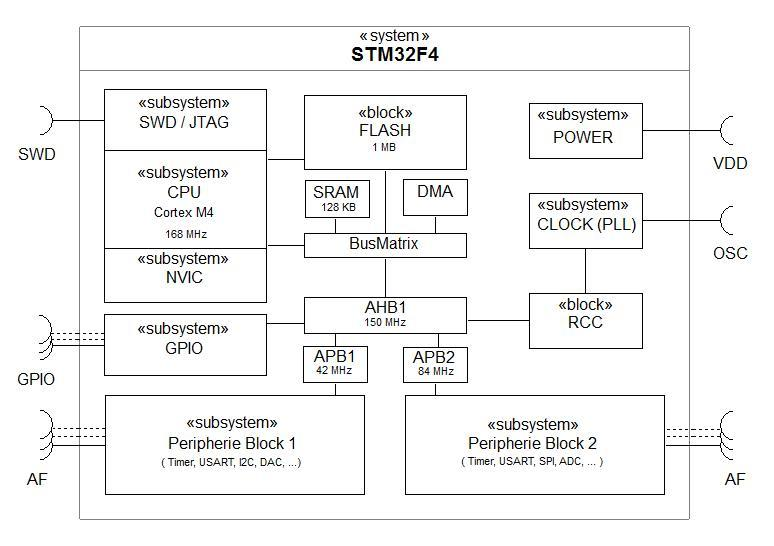
\includegraphics[width=400px,height=300px]{../img/stm32f4_prinzip.jpeg}
	\caption{Simple M4 Diagram}
	\label{m4_simple}
\end{figure}

The diagram doesn't show, which peripheral systems are connected to which
APBX-Bus, but that can be seen in the datasheet. What it does show is, that
the GPIO-Pins, are connected to the AHB1-Bus.\\
The reason for that is, that it's much faster then what is recommended
 for most the part of what a GPIO demands. The subsystems on the other hand aren't
 necessarily needed to react that fast.\\

For example the USART6, which is used in the project, is connected to APB2.
A much more precise representation of the STM32F4 is illustrated in the following diagram.\\

The AHB1 is the system bus and therefore should be really fast.
\includepdf[pages={18}]{../img/blockdia.pdf}

The peripheral systems are addressed through the busses. For example the
GPIOA and USART6.
The address range of the peripherals is 0x4000\_0000 - 0x5FFF\_FFFF. The
peripheral base address is 0x4000\_0000. To configure and write to / read from
the USART6 we need the peripheral base address and an offset. In the case of
USART6 the offset is a combination of two offsets, as seen in the table:
\includepdf[pages=73]{../img/blockdia.pdf}
\begin{enumerate}
	\item Peripheral Base: 0x40000000
	\item APB2: Peripheral Base + 0x10000 = 0x40010000
	\item USART6\_Base: APB2 + 0x1400 = 0x40011400
\end{enumerate}

At the USART6\_Base is equal to the USART Status register. To transceive data
via USART6 the DR register (16-bit) with an additional offset of 0x04 is right
one.

It is one register to read to and write from. That is a good example, why an
interrupt handler is needed (NVIC). The program would have a huge timing problem
since the read operation on that register would cause a huge delay, because
it would wait till data is read.

On this way all the peripherals are can be addressed.
For the GPIOA it is theoretically the same but with other addresses. The GPIOA
is connected via the faster AHB1 bus.
\begin{enumerate}
	\item AHB1\_Base: Peripheral Base + 0x20000
	\item GPIOA\_Base: AHB1\_Base
\end{enumerate}
These are just two examples of the addressing of the ARM peripherals, but at the
bottom they are all the same - it's all about the addresses.
